\chapter{Measurement of differential single-top-quark cross sections at 13~TeV}
\label{ch:diff13}

\intro{A first measurement of normalized differential single-top-quark cross sections in $t$~channel as a function of the top quark transverse momentum and rapidity at 13~\TeV is presented. \Acrlong{pp} collision data corresponding to an integrated luminosity of 2.3~\invfb are analyzed which were recorded in 2015 with the \gls{cms} experiment. Events containing one isolated muon and two or three jets are selected and a \acrlong{bdt} is trained for separating signal from background events further. The amount of signal events as a function of the top quark transverse momentum and rapidity is estimated by multiple fits. The results are unfolded to parton level and compared to predictions by various \acrlong{mc} generators. No significant deviations are observed. The measurement has been published in Ref.~\cite{CMS-PAS-TOP-16-004}.
}

%##############################################
\section{Analysis strategy}
%##############################################

In the following, the strategy for measuring normalized differential single-top-quark cross sections in $t$~channel as a function of the top quark \pt and rapidity is outlined. Events containing one isolated muon and two or three jets are selected. Then, a \gls{bdt} is trained to obtain a powerful discriminant for separating signal from background events. The amount of signal and background events in data are estimated by fitting the distributions of the transverse W~boson mass and the \gls{bdt} discriminant in the signal and in two \ttbar-dominated control regions simultaneously. Additionally, the contamination by multijet events is also estimated using a data-driven template of its shape obtained from a sideband region, for which the muon isolation during the event selection is inverted. Multiple fits are performed in intervals of the top quark transverse momentum and rapidity. The differential cross sections are inferred by passing the fit results directly to the unfolding. The impact of systematic uncertainties on the differential cross section is evaluated by repeating the measurement with modified templates.

\todo{not good here}
The strategy has multiple benefits compared to the one chosen for the polarization measurement~(Ch.~\ref{ch:polarization}). First, it is not necessary to define a signal-enriched region where the remaining backgrounds are subtracted from data prior to unfolding. Instead, the signal yields in intervals of the top quark \pt and rapidity are taken from the fits directly. Secondly, since no signal-enriched region is defined also optimization of its selection is required. No explicit selection to reject multijet events or on the \gls{bdt} discriminant is necessary to carry out the measurement. Only for validation purposes, events with $\mtw>50~\GeV$ are selected to verify the modeling of background processes in a multijet-depleted region. Lastly, residual differences in the estimated backgrounds yields between unfolding bins are profiled which reduces the impact by potential shortcomings in their modeling or a bias occurring through correlations of \gls{bdt} input observables with the top quark \pt and rapidity.

The measured normalized cross sections are compared to the predictions by various event generators.

%##############################################
\section{Event selection and simulated samples}
%##############################################

The measurement is based on \gls{pp} collision events corresponding to 2.3~\invfb which were recorded by the \gls{cms} experiment in 2015 at a \acrlong{cm} energy of 13~\TeV. An isolated muon trigger is employed for recording data events which requires the presence of an isolated muon candidate with a transverse momentum of at least $20~\GeV$ within $|\eta|<2.4$. In the analysis, the muon candidate has to have a momentum of $\pt>22$ within $|\eta|<2.4$ and fulfill tight identification requirements. The muon candidate is required to be isolated with a relative \gls{deltabeta}-based isolation of $\muiso<6\%$, calculated from the transverse energy deposits of charged and neutral hadrons, photons, and tracks associated to pileup within a cone of $\Delta R<0.4$. The isolation is explicitly chosen tighter here compared to corresponding analyses at 8~\TeV (e.g. Ch.~\ref{ch:polarization}) in which $\muiso<12\%$ was required instead. The distribution of the relative muon isolation after applying the complete event selection with the exception of the isolation is presented in Fig.~\ref{fig:diff13-reliso}. Here, the multijet template is taken exceptionally from simulation and scaled such that it fits to the bulk of the data distribution. The deviation at high isolation values can be attributed to differences in the trigger turn-on efficiencies between simulation and data. The distribution motivate to choose a tighter isolation here to counter observed the larger contamination by multijet events at 13~\TeV.

\myfigure{\label{fig:diff13-reliso} Distribution of the relative \gls{deltabeta}-based muon isolation in 2j1t. The multijet template is taken from simulation.}{
\subfloat[]{\adjincludegraphics[height=4.8cm,trim={0 0 {0.\width} 0},clip]{figures/differential/plots/2j1t/2j1t_relIso_qcdnone.pdf}}
}

Processes with $\mu\mu\mathrm{\mbox{+}jets}$ or $\mu\mathrm{e}\mathrm{\mbox{+}jets}$ final states such as dileptonic \ttbar or \zjets production are suppressed by vetoing events containing additional muon candidates with $\pt>10~\GeV$ within $|\eta|<2.5$ or electron candidates with $\pt>20$ within $|\eta|<2.5$ that also corresponding fulfill loose identification criteria.

\Gls{pf} candidates are clustered into jets using the anti-\kt algorithm with a distance parameter of $R=0.4$. The influence by pileup is mitigated through the \gls{chs} technique~\cite{CMS-PAS-JME-14-001}. The jet energy scale is corrected in data and simulation using dedicated (\pt,$\eta$)-dependent scale factors. Additionally, the jet energy resolution is corrected in simulation to match the one observed in data. After these corrections are applied, jets with a transverse momentum of at least $40~\GeV$ that fall within $|\eta|<4.7$ and fulfill loose identification requirements are selected for analysis. A potential overlap between selected jets and the tight muon is removed by ignoring jets that fall within a cone of $\Delta R<0.3$ around the selected muon candidate. The \acrfull{csv} algorithm (version~2) is employed to perform b-tagging. At its tight working point an efficiency for tagging true b~jets of about 50\% is achieved whereas the misidentification rate amounts to only 0.1\%~\cite{CMS-PAS-BTV-15-001}. Simulated events are reweighted to match the observed b-tagging efficiency in data using dedicated scale factors.

The following samples of simulated events are employed in the measurement. The \MGAMC generator interfaced with \PYTHIA8 for hadronization is used to generate the default signal sample of $t$-channel single-top-quark production in 4~\gls{fs}. For comparison, alternative samples are generated using the \MGAMC generator interfaced with \PYTHIA8 in 5~\gls{fs}, \MGAMC interfaced with \HERWIG in 4~\gls{fs}, and the \POWHEG generator interfaced with \PYTHIA in 4~\gls{fs}. Single-top-quark production in tW-channel and \ttbar production are simulated using the \POWHEG generator interfaced with \PYTHIA8. The samples of \wjets and \zjets production are generated using \MGAMC interfaced with \PYTHIA8 as well. The contributions by single-top-quark production in $s$~channel and diboson production have been found negligible at 13~\TeV and corresponding samples are thus not utilized. The theoretical cross sections for normalizing these samples are listed in Tab.~\ref{tab:diff13-theo-xsecs}. Special care needs to be taken for normalizing the samples produced with the \MGAMC generator because the \gls{mcatnlo} matching scheme has been employed here which leads to a certain fraction of negatively weighted events.

\mytable{\label{tab:diff13-theo-xsecs}Theoretical cross sections used to normalize the simulated samples.}{
\begin{tabular}{|l  r c l |}
\hline
process & cross section &\hspace{0.05cm} & accuracy \\
\hline
$t$~channel top quark & $136.0^{+5.4}_{-4.6}~\pb$ && \gls{nlo} (using \HATHOR\,2.1~\cite{Aliev:2010zk})   \\
$t$~channel top antiquark & $81.0^{+4.1}_{-3.6}~\pb$ && \gls{nlo} (using \HATHOR\, 2.1~\cite{Aliev:2010zk})   \\
tW~channel & $71.7\pm3.8~\pb$ && \gls{nlo} (using \HATHOR\,2.1~\cite{Aliev:2010zk})  \\
\ttbar & $832^{+20}_{-29}~\pb$ && \gls{nnlo} (using \TOPPP\,2.0~\cite{Czakon:2011xx}) \\
$\mathrm{W}\to\ell\nu\mathrm{\,\mbox{+}\,jets}$ & $20\,509^{+788}_{-776}~\pb$ && \gls{nnlo} (using \FEWZ\,3.1~\cite{Li:2012wna}) \\
$\mathrm{Z}/\gamma^{*}\to\ell^{\rmplus}\ell^{\rmminus}$, $m_{\ell\ell}>50~\GeV$ & $2\,008^{+76}_{-75}~\pb$ && \gls{nnlo} (using \FEWZ\,3.1~\cite{Li:2012wna}) \\
\hline
\end{tabular}
}

The shape of multijet events is modeled using a template \ref{sec:diff13-fit} ???

\myfigure{\label{fig:diff13-mtw-antiiso} Distributions of the transverse W boson mass: (a)~sideband region with inverted muon isolation; (b)~signal region.}{
\subfloat[]{\adjincludegraphics[height=4.8cm,trim={0 0 {0.16\width} 0},clip]{figures/differential/antiiso/2j1t_mtw_qcdnone_nol.pdf}}
\subfloat[]{\adjincludegraphics[height=4.8cm,trim={0 0 {0.\width} 0},clip]{figures/differential/plots/2j1t/2j1t_mtw_qcdnone.pdf}}
}

Similar to the polarization measurement, signal and control regions are defined based on the number of selected jets and the subset of jets which are also b-tagged. Distributions of the reconstructed top quark mass in signal and control regions after applying the event selection are presented in Fig.~\ref{fig:diff13-topmass}. Since the 3j2t region contains a relatively low number of events, the 3j1t region is considered as an additional \ttbar control region in this analysis.

 
\myfigure{\label{fig:diff13-topmass} Distributions of the reconstructed top quark mass in signal and control regions.}{
\subfloat[]{\adjincludegraphics[height=4.8cm,trim={0 0 {0.16\width} 0},clip]{figures/differential/plots/2j0t/2j0t_top_mass_qcdnone_nol.pdf}}
\subfloat[]{\adjincludegraphics[height=4.8cm,trim={0 0 {0.\width} 0},clip]{figures/differential/plots/2j1t/2j1t_top_mass_qcdnone.pdf}}\\
\subfloat[]{\adjincludegraphics[height=4.8cm,trim={0 0 {0.16\width} 0},clip]{figures/differential/plots/3j1t/3j1t_top_mass_qcdnone_nol.pdf}}
\subfloat[]{\adjincludegraphics[height=4.8cm,trim={0 0 {0.\width} 0},clip]{figures/differential/plots/3j2t/3j2t_top_mass_qcdnone.pdf}}
}


%##############################################
\section{Modeling}
%##############################################
\label{sec:diff13-modeling}
Njets, Nbjets, tune studies
show cosTheta in 2j0t for wjet modeling for amc and mg samples if possible, qcd


%##############################################
\section{BDT training}
%##############################################
\label{sec:diff13-bdt}

%##############################################
\section{Signal extraction}
%##############################################
\label{sec:diff13-fit}


%##############################################
\section{Unfolding}
%##############################################

%##############################################
\section{Results}
%##############################################


%##############################################
\section{Prospects}
%##############################################

%##############################################
\subsection{Extended samples}
%##############################################

%##############################################
\subsection{Fiducial studies}
%##############################################
\label{sec:diff13-fiducial-studies}



Figures~\ref{fig:technique-particle-level-muonpt} and~\ref{fig:technique-particle-level-muoneta} show a comparison of the muon $\pt$ and pseudorapidity at reconstruction, particle, and parton level after selecting events with one muon at each level respectively. The top panels demonstrate a high overlap of the events selected at reconstruction level with the ones at particle and parton level. The acceptance rises with the muon momentum from about 40\% to 90\% due to the relative isolation requirement for reconstructed muons. The number of jets is presented in Fig.~\ref{fig:technique-particle-level-njet}. Due to the jet energy scale correction, 


dressed leptons (cone algorithms associates photons to leptons but does not cluster close leptons), tau decays, jet clustering (no neutrinos/leptons), b-tagging,




particle level overlap: tightMu: >99\%, 2jets: 80\%, 2j1t: 70\%


\myfigure[p]{\label{fig:technique-particle-level}Comparison of expected event densities for $1~\invfb$ at $13~\TeV$ after applying the event selection at reconstruction, particle, and parton level respectively:  (a)~muon $\pt$, (b)~muon rapidity, and (c)~number of jets after requiring one isolated and tight muon; (d)~number of b-tagged jets, (e)~$\pt$ and (f)~pseudorapidity of the spectator jet after requiring one isolated, tight muon and two jets where in (e,f) one jet is additionally required to be b-tagged at reconstruction level. Top panels show the common events selected at reconstruction level while the bottom panels display the acceptance.}{
\subfloat[\label{fig:technique-particle-level-muonpt}]{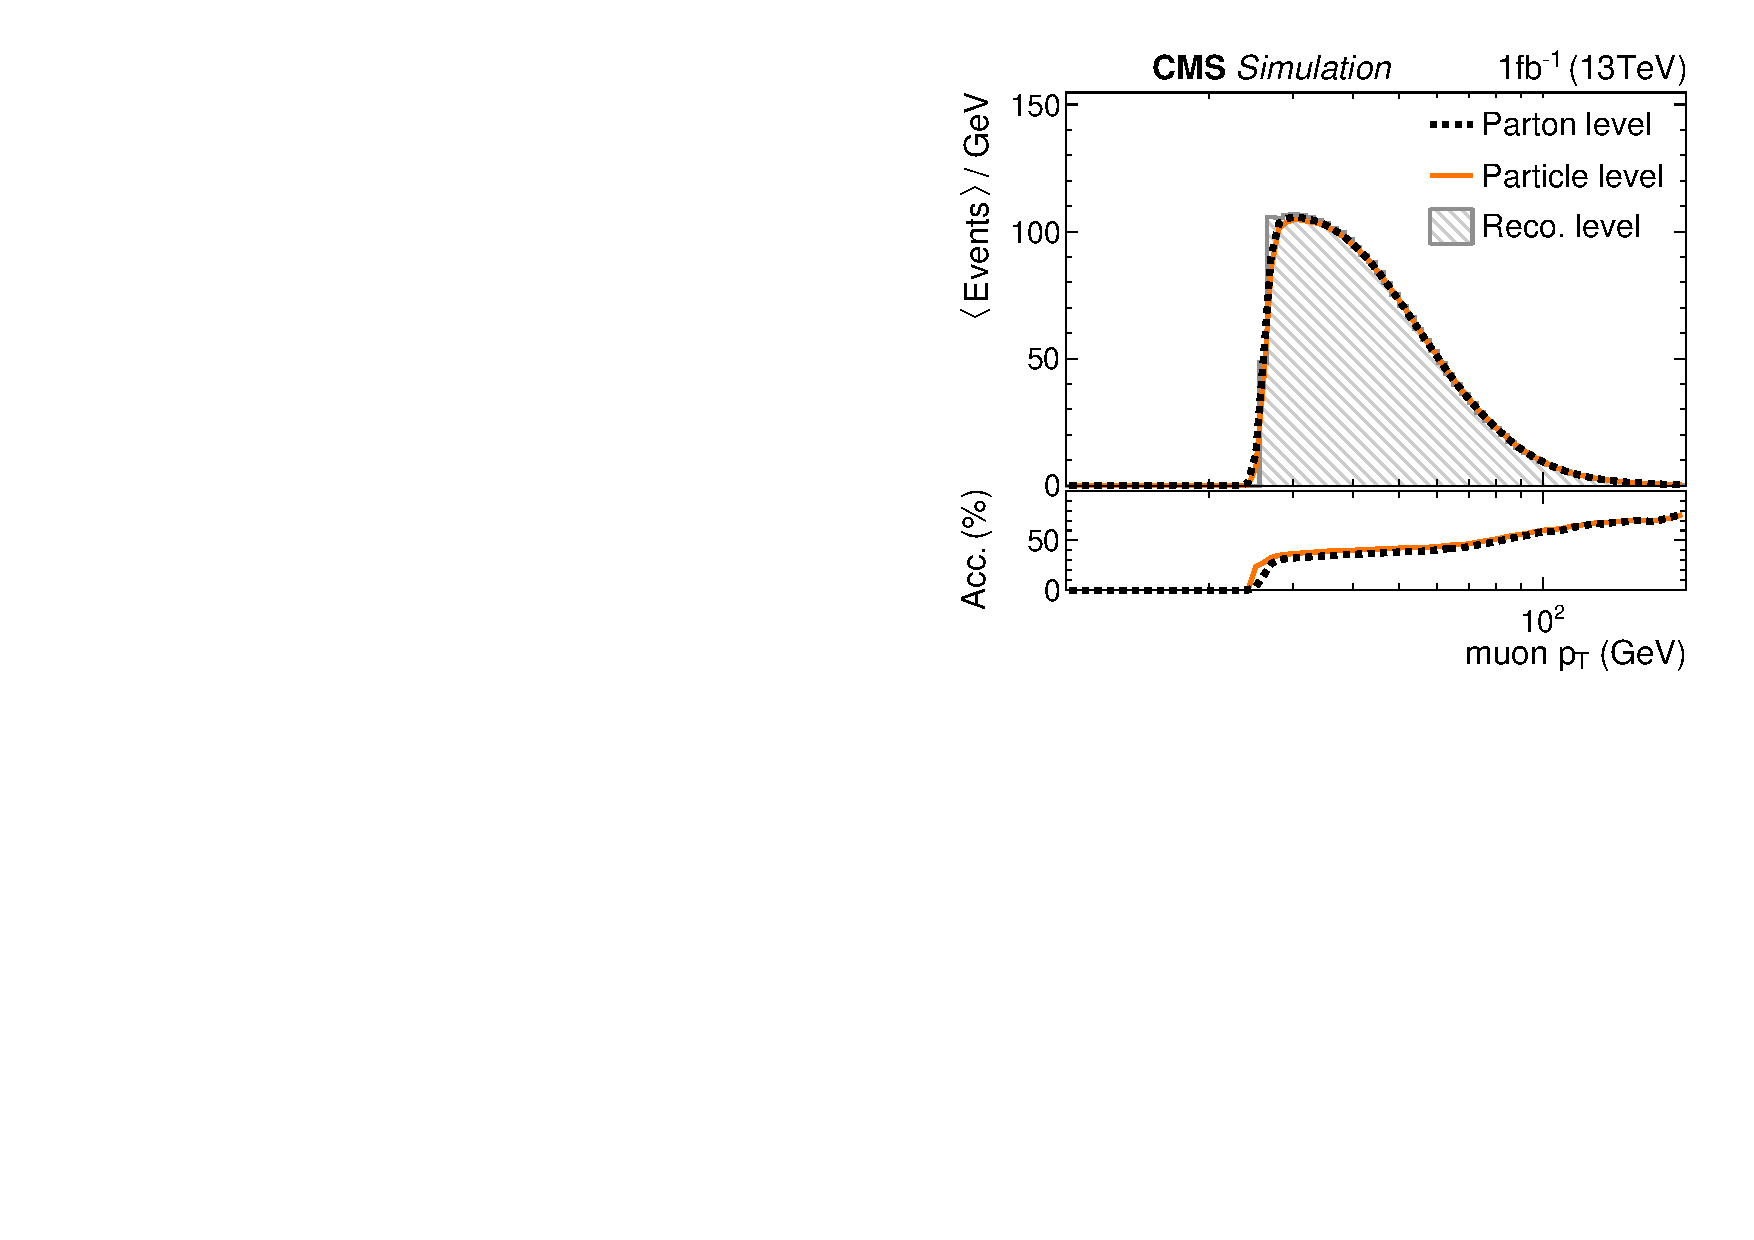
\includegraphics[width=0.48\textwidth]{figures/technique/muon_particle_logpt.pdf}}\hspace{0.03\textwidth}
\subfloat[\label{fig:technique-particle-level-muoneta}]{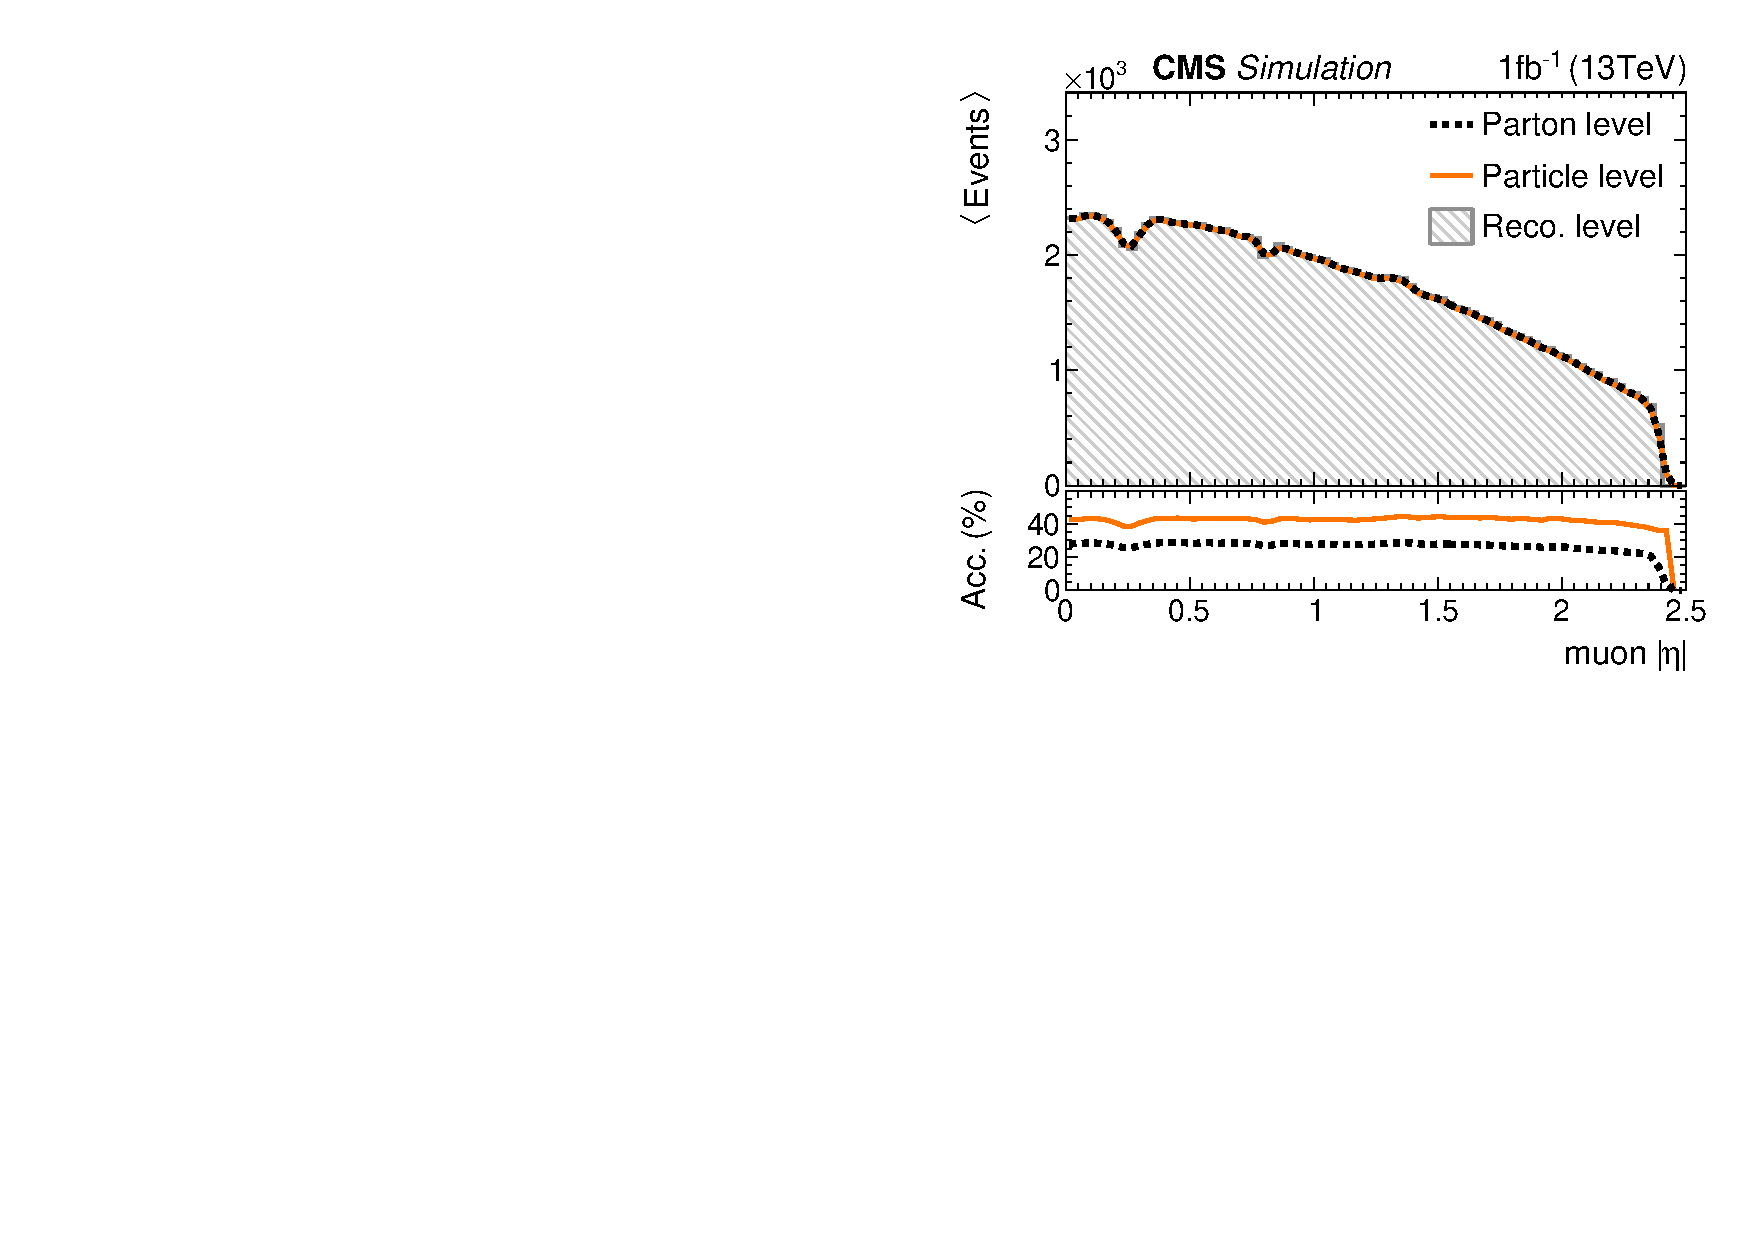
\includegraphics[width=0.48\textwidth]{figures/technique/muon_particle_abseta.pdf}}\\
\subfloat[\label{fig:technique-particle-level-njet}]{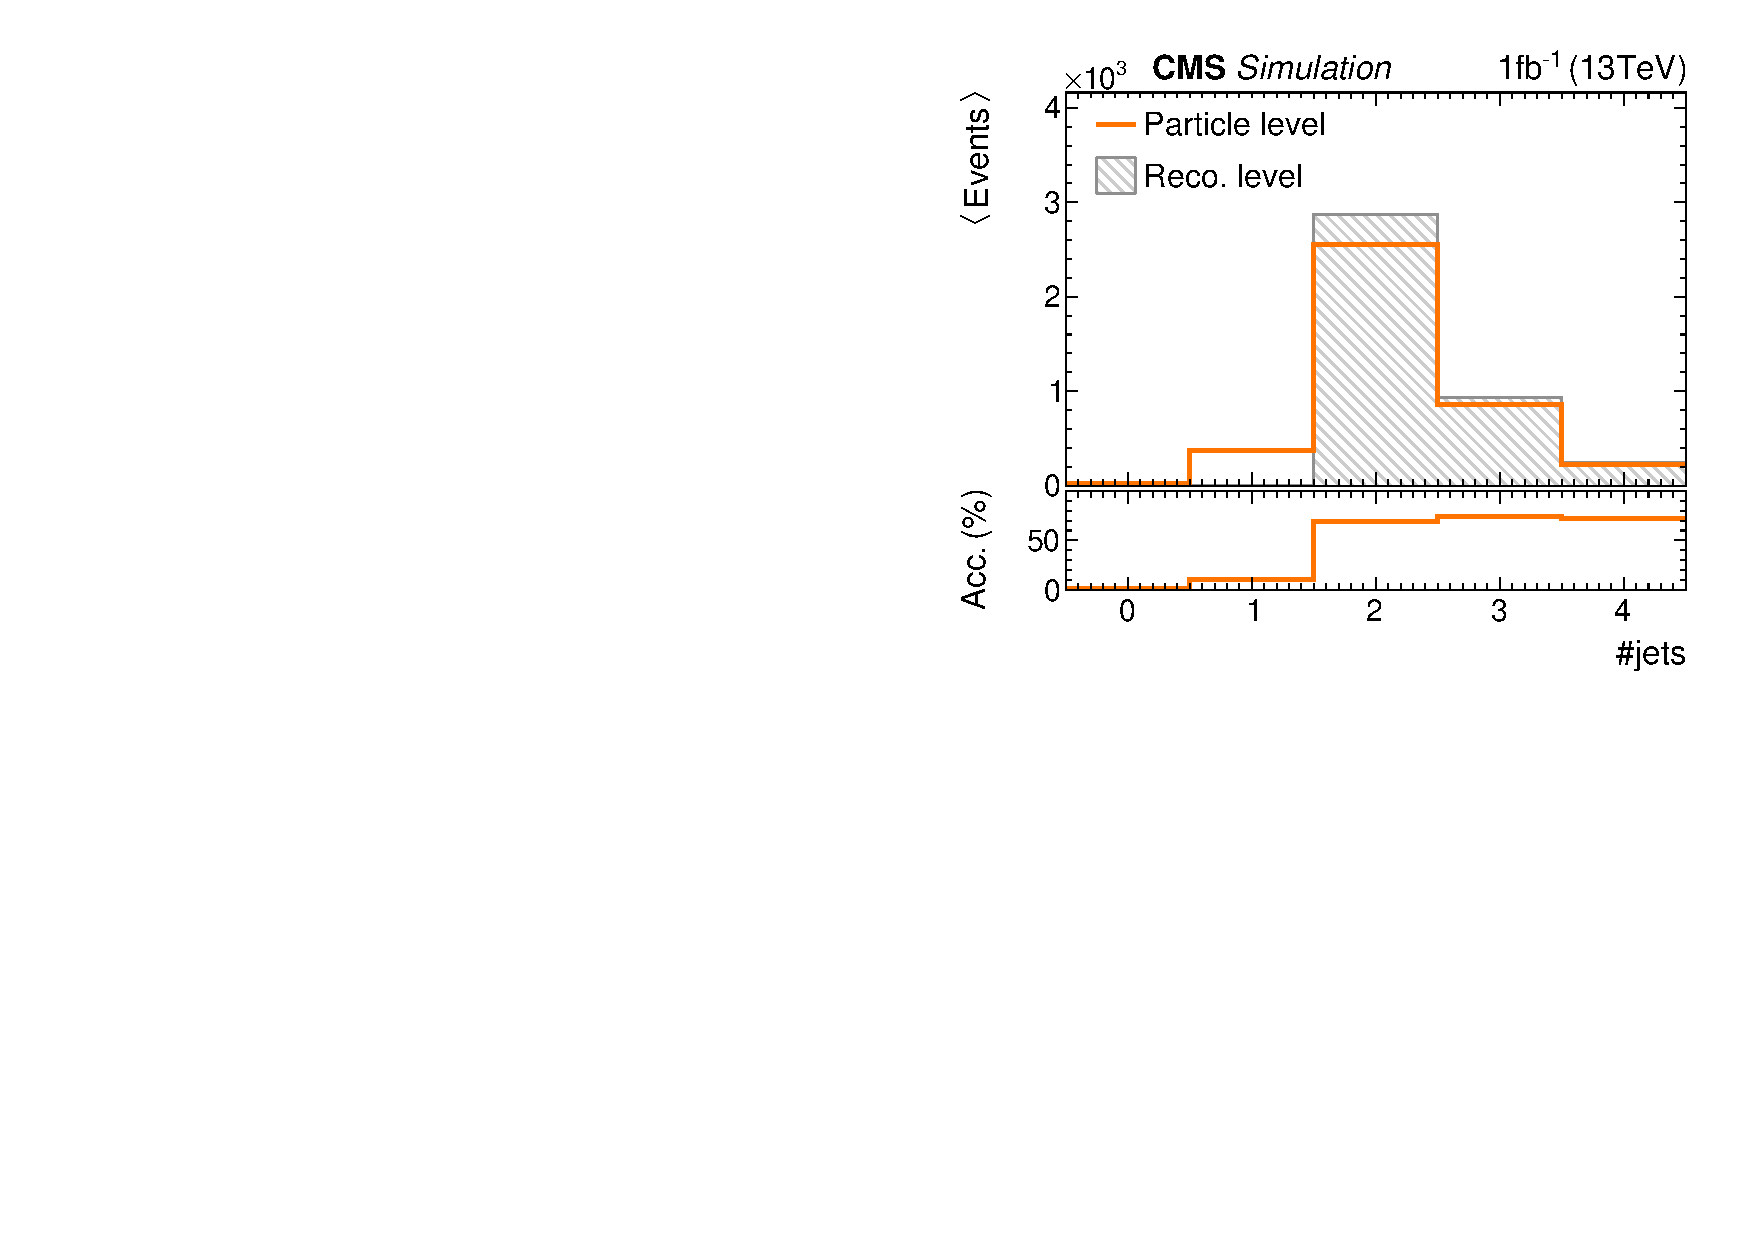
\includegraphics[width=0.48\textwidth]{figures/technique/njet_particle.pdf}}\hspace{0.03\textwidth}
\subfloat[\label{fig:technique-particle-level-nbjet}]{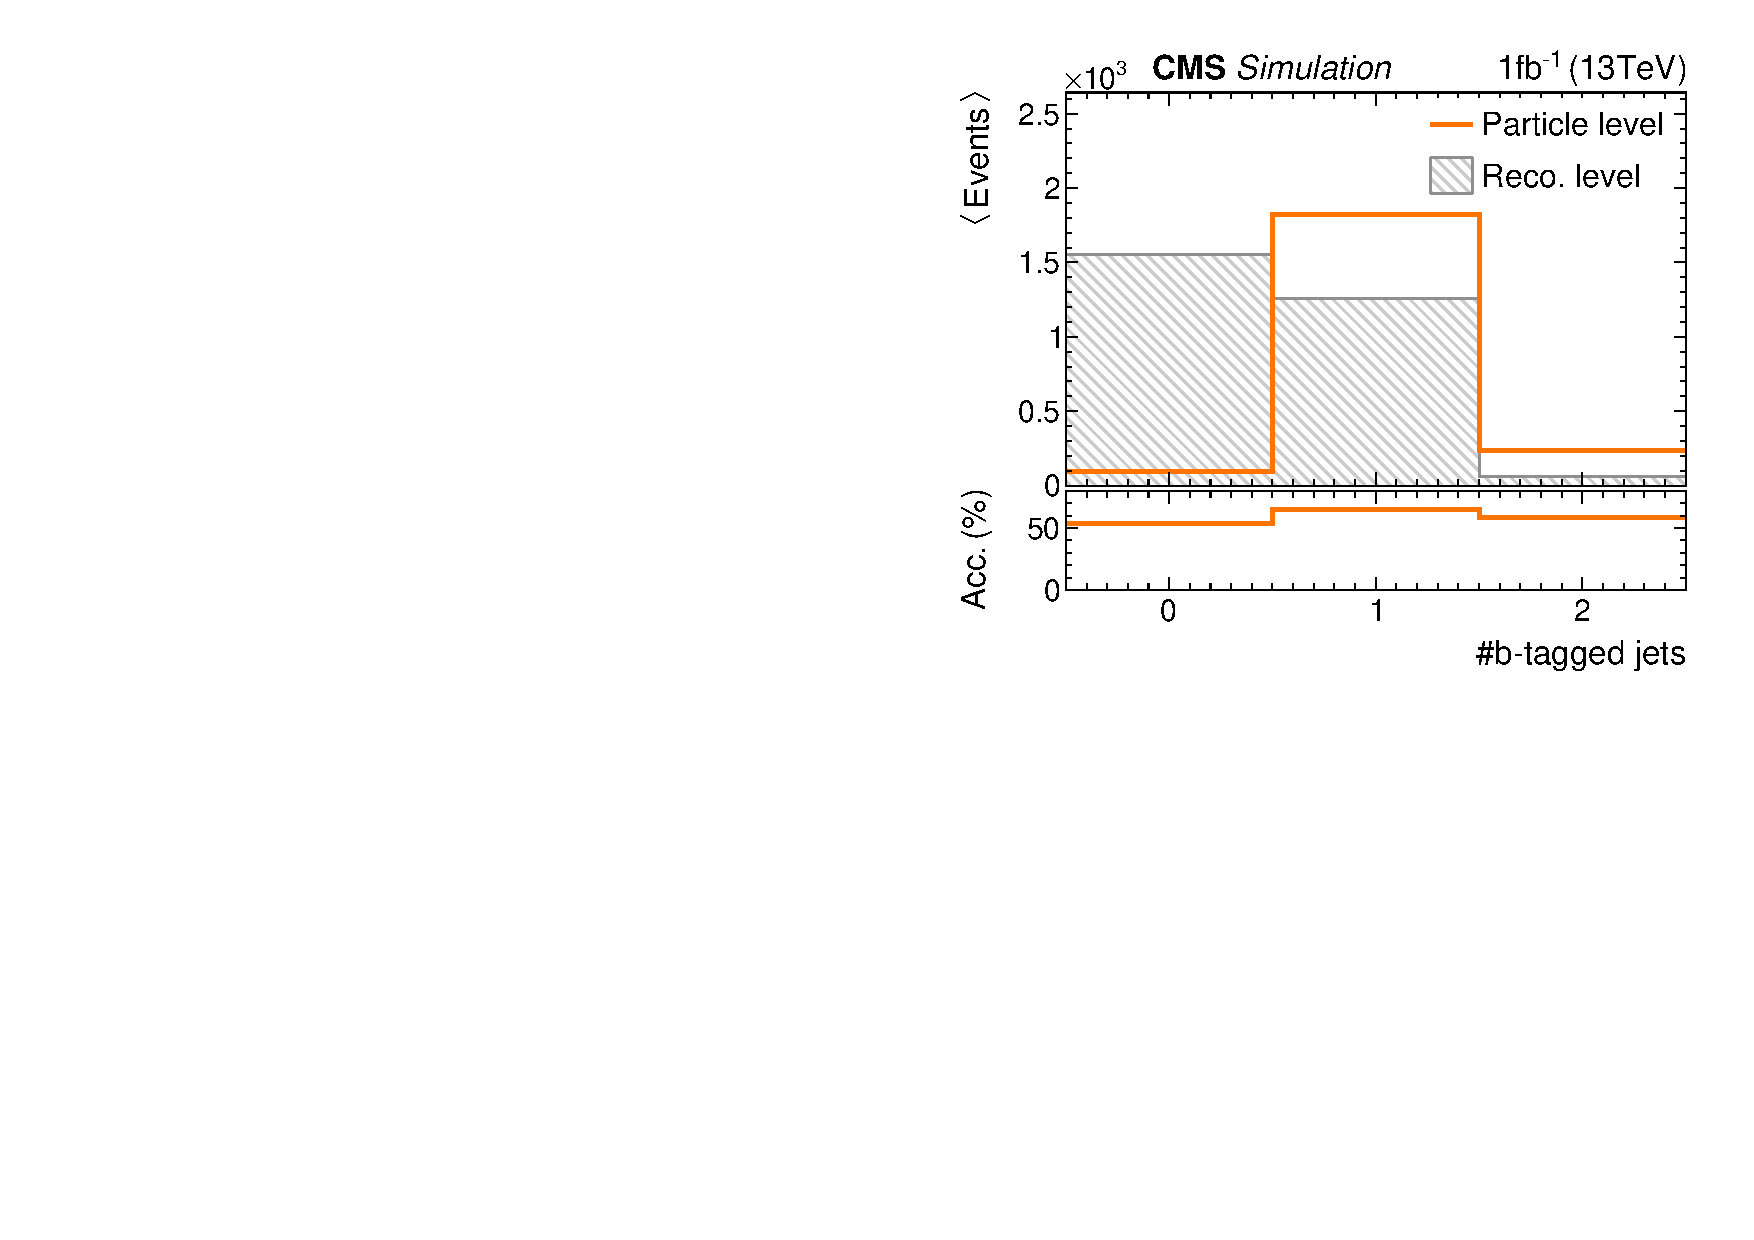
\includegraphics[width=0.48\textwidth]{figures/technique/nbjet_particle.pdf}}\\
\subfloat[\label{fig:technique-particle-level-ljetpt}]{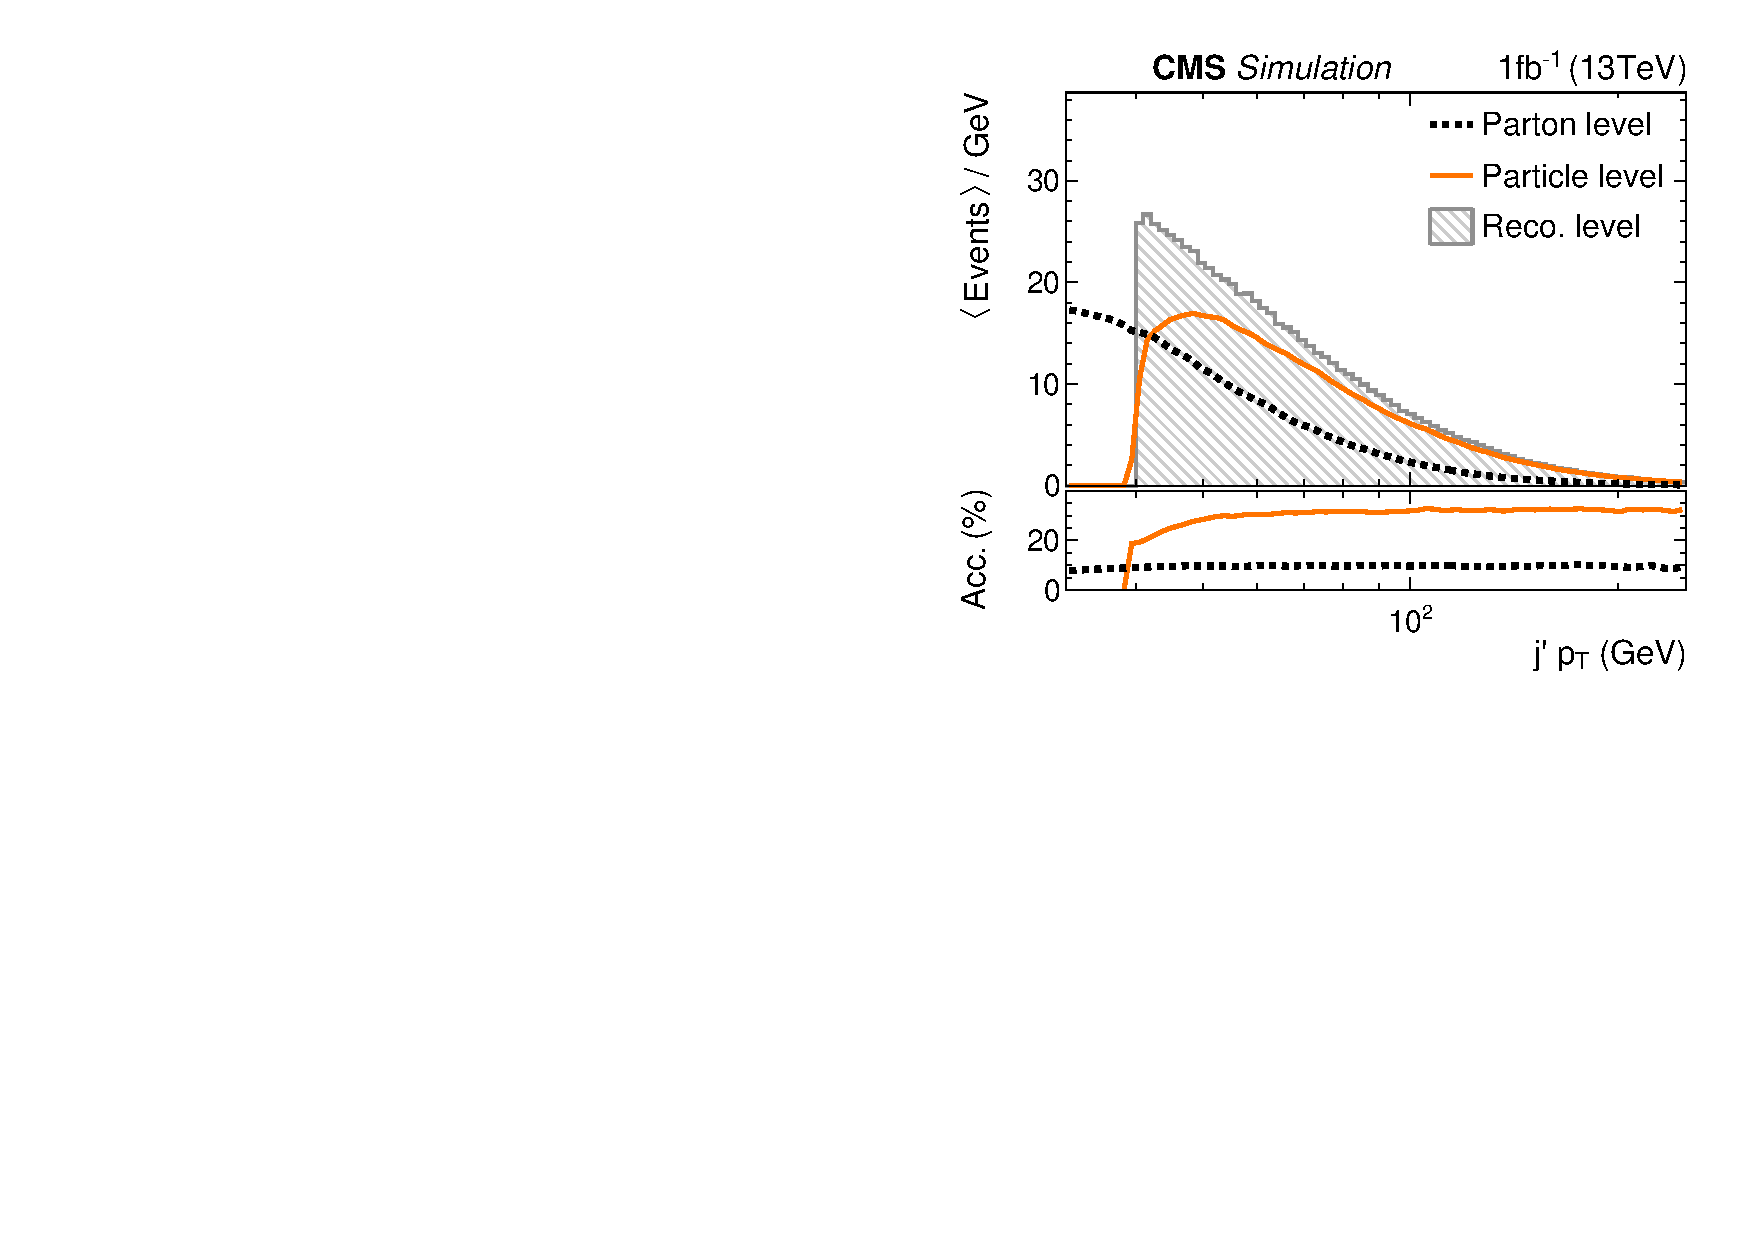
\includegraphics[width=0.48\textwidth]{figures/technique/ljet_particle_logpt.pdf}}\hspace{0.03\textwidth}
\subfloat[\label{fig:technique-particle-level-ljeteta}]{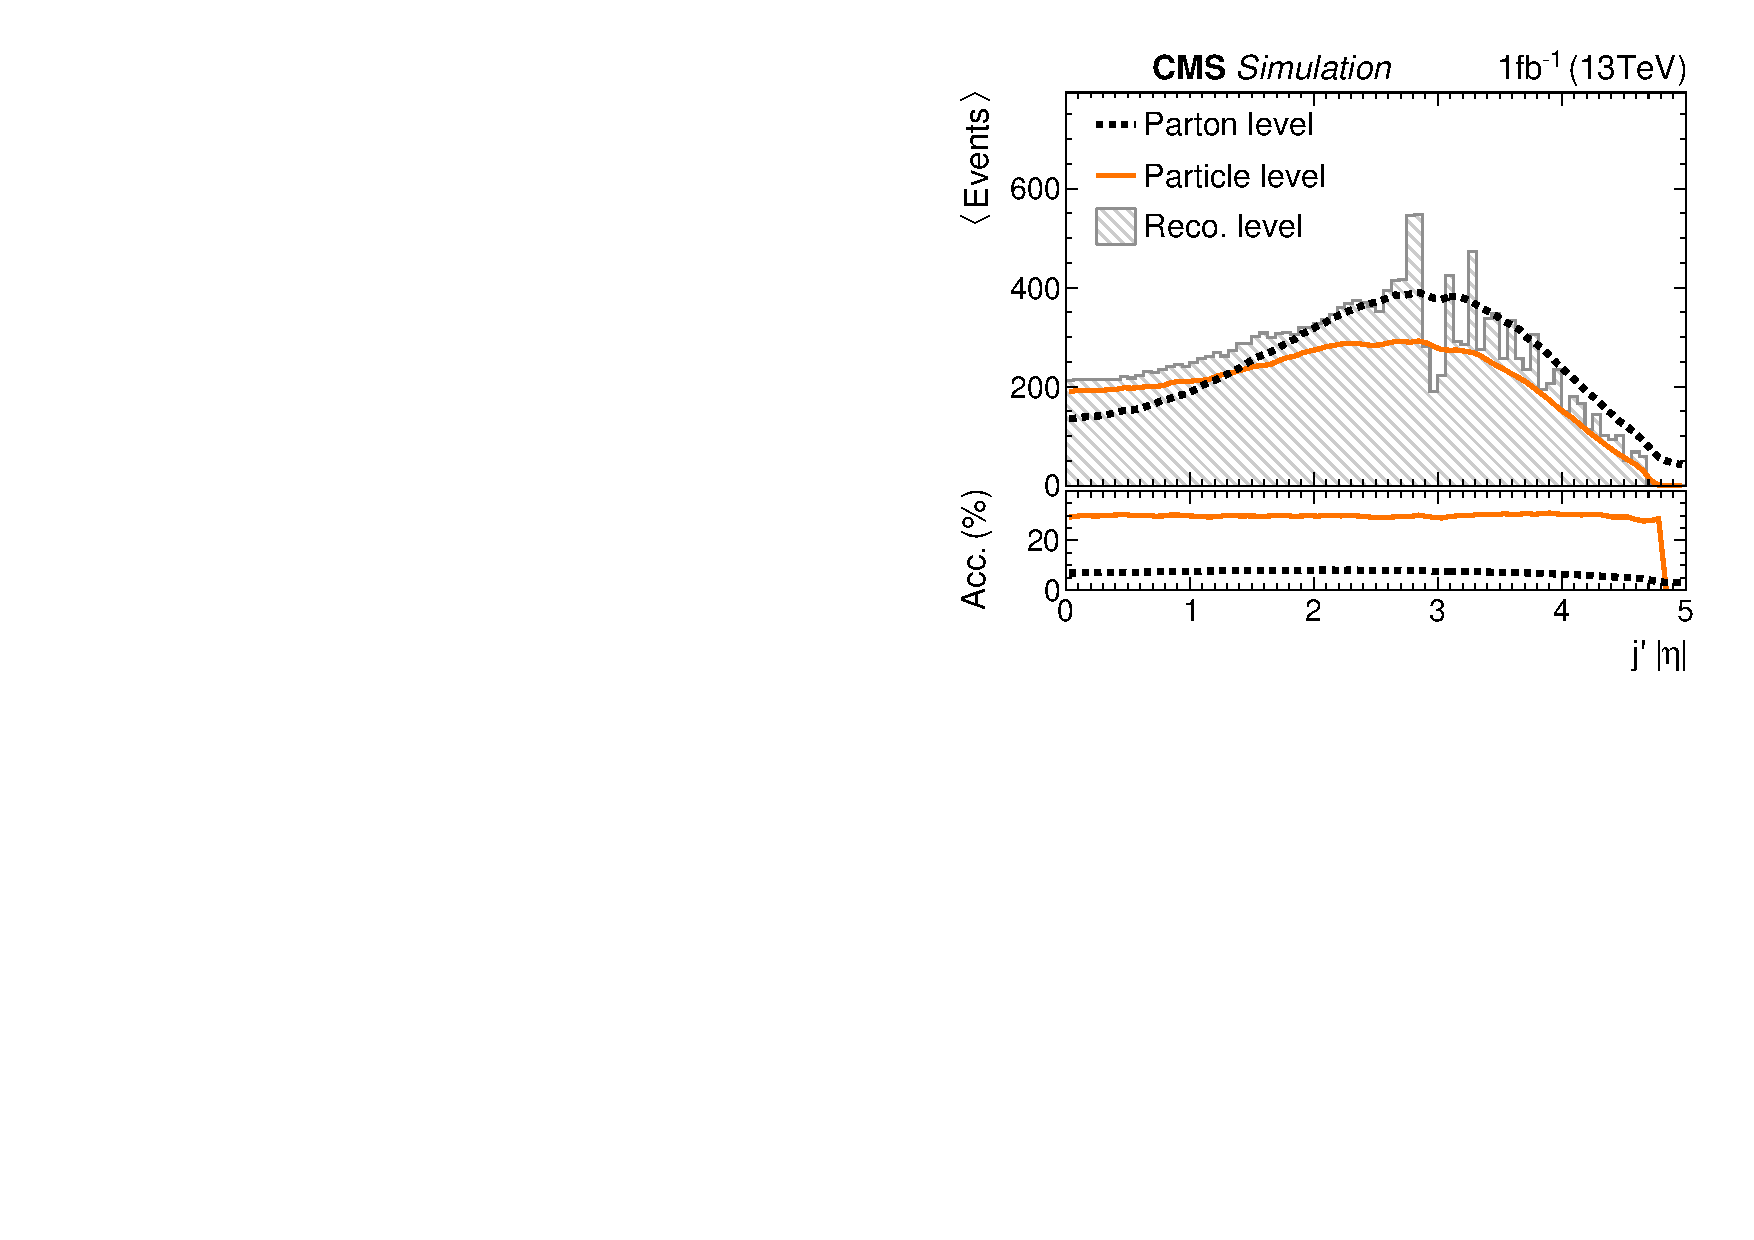
\includegraphics[width=0.48\textwidth]{figures/technique/ljet_particle_eta.pdf}}
}

\myfigure[phtb]{\label{fig:technique-particle-top}Comparison of event selection at reconstruction and particle level.}{
\subfloat[]{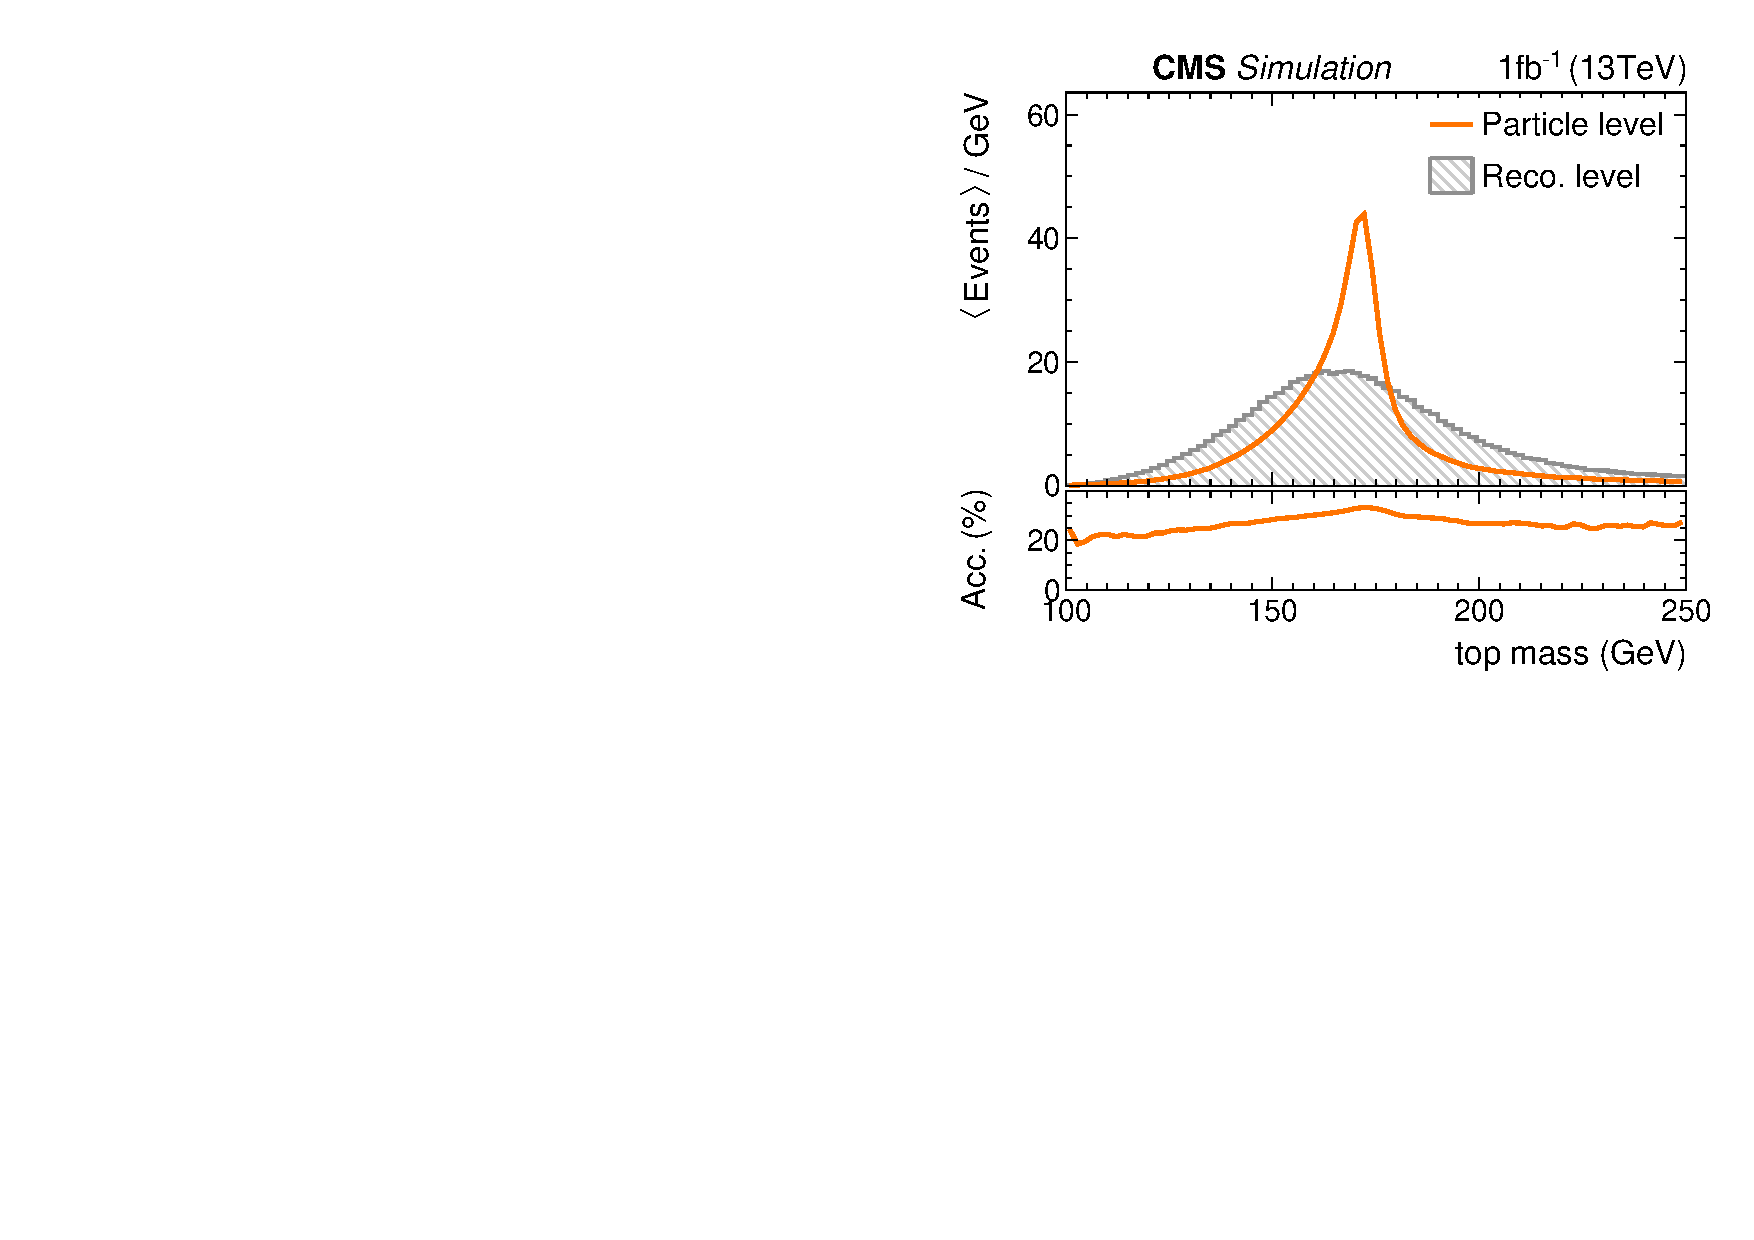
\includegraphics[width=0.48\textwidth]{figures/technique/top_particle_mass.pdf}}\hspace{0.03\textwidth}
\subfloat[]{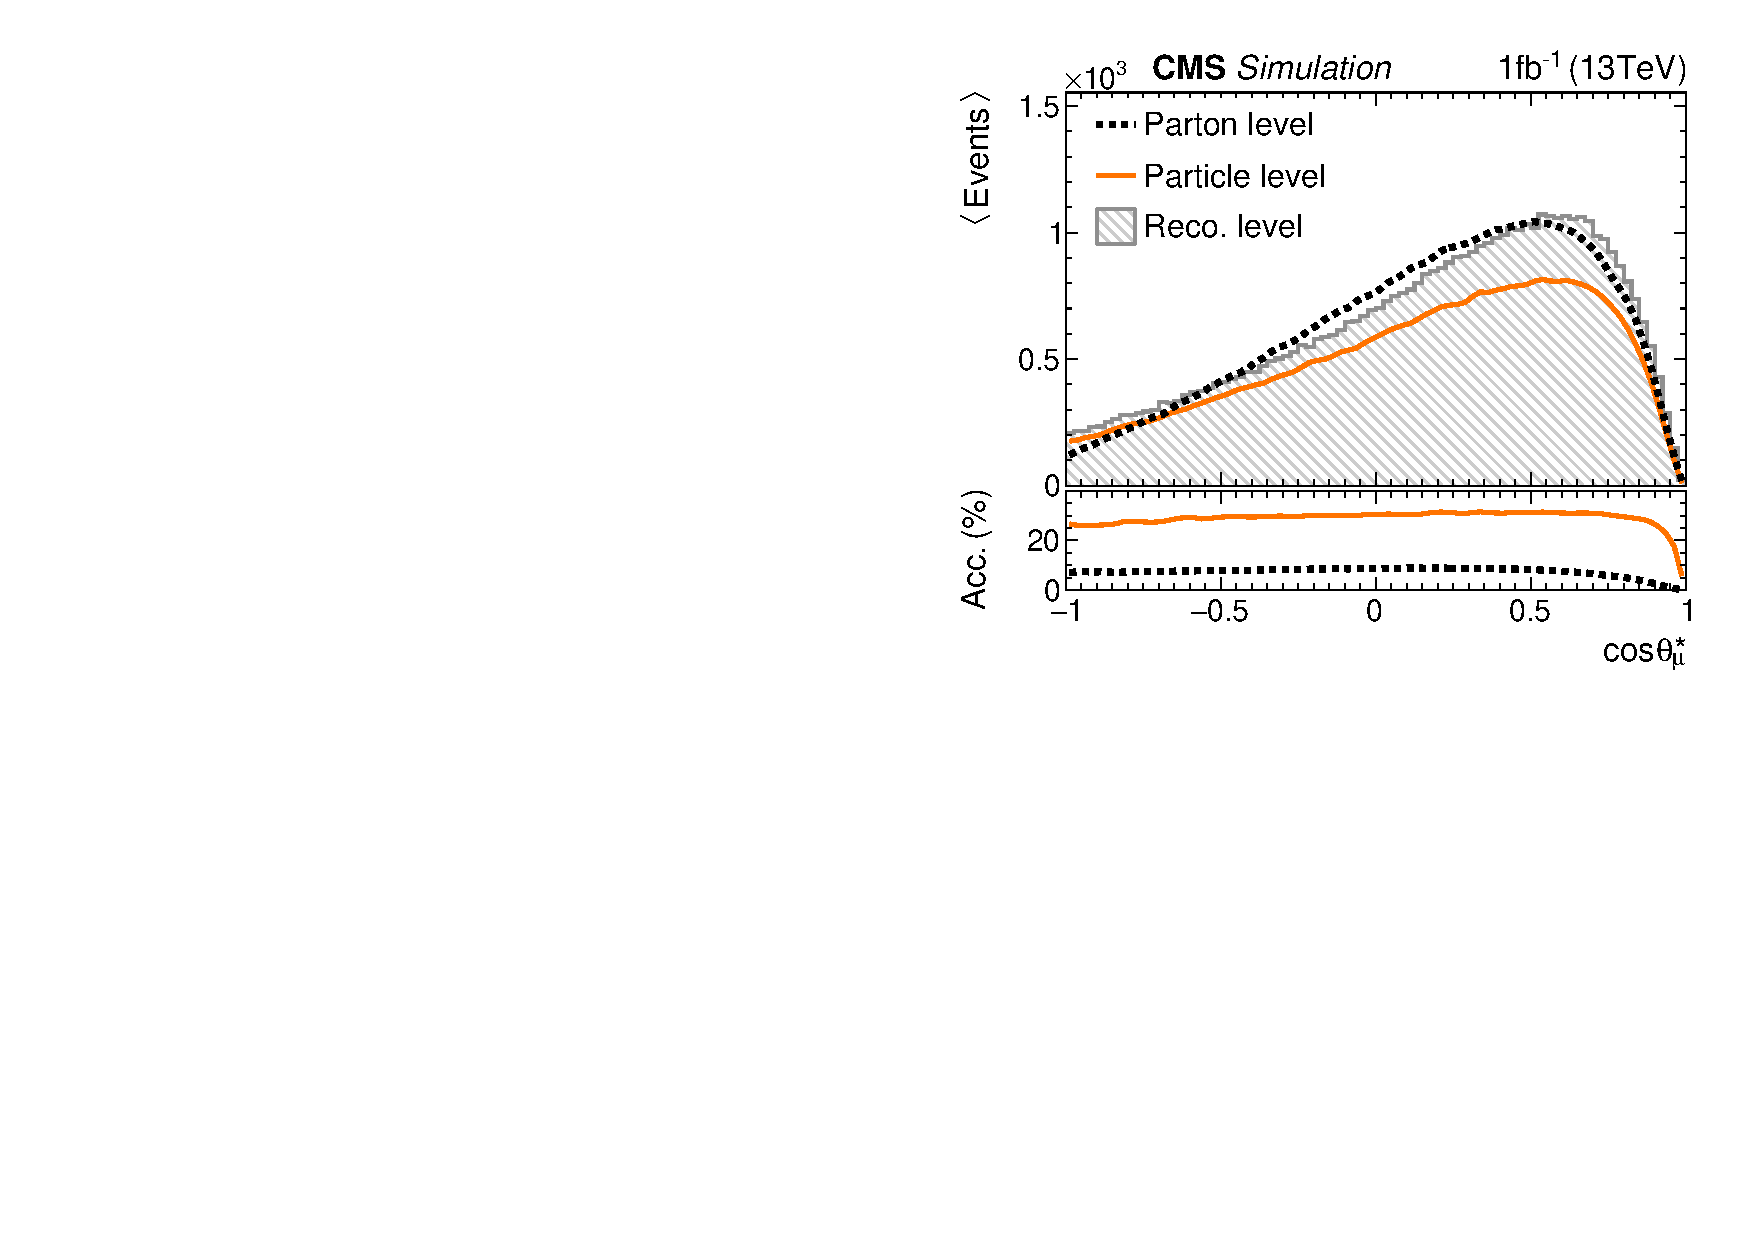
\includegraphics[width=0.48\textwidth]{figures/technique/cosTheta_particle.pdf}}
}
